%%%%%%%%%%%%%%%%%%%%%%%%%%%%%%%%%%%%%%%%%%%%%%%%%%%%%%%%%%%%%%%%%%%%%%%%
%                                                                      %
%     File: Thesis_Implementation.tex                                  %
%     Tex Master: Thesis.tex                                           %
%                                                                      %
%     Author: Andre C. Marta                                           %
%     Last modified :  2 Jul 2015                                      %
%                                                                      %
%%%%%%%%%%%%%%%%%%%%%%%%%%%%%%%%%%%%%%%%%%%%%%%%%%%%%%%%%%%%%%%%%%%%%%%%

\chapter{Implementation}
\label{chapter:implementation}

This section will go in depth on the implementation of the concepts presented in the chapter \ref{chapter:background}. The plane model to be controlled was firstly implemented and verified. The first goal after this first step was to design a controller that would allow the aircraft to follow a trajectory from several position waypoints through time. The influence of certain parameters and knowledge of the exact plane model will be studied and discussed in chapter \ref{chapter:results}. The final goal will be to improve the controller and its robustness by reducing tracking error through the use of an adaptive neural network.

%%%%%%%%%%%%%%%%%%%%%%%%%%%%%%%%%%%%%%%%%%%%%%%%%%%%%%%%%%%%%%%%%%%%%%%%
\section{Plane Model}
\label{section:model}

The chosen commercial aircraft that will be simulated is the Boeing 737-200, an aircraft with over 30 years of service for which information of flight parameters is readily available. The simulation was made in a cruise flight environment, at $200$ m/s velocity at $10000$ m above the ground. The chosen inertial matrix for this aircraft is given by
\begin{equation}
\begin{bmatrix}
1278369.56 & 0 & -135588.17\\
0 & 3781267.79 & 0\\
-135588.17 & 0 & 4877649.98
\end{bmatrix}
\end{equation}
The ISA atmospheric model was used to measure the air density at any given height.
\begin{table}[htbp]
  \centering
  \caption{Boeing 737-2 parameters}
    \begin{tabular}{rr}
    \toprule
    Weight $m$ & $52390$ kg \\
    Wing Span $b$ & $28.35$ m \\
    Wing Area $S$ & $102.0$ m$^{2}$ \\
    Wing mean chord $\bar{c}$ & $4.35$ m \\
    Length $l$ & $30.53$ m \\
    \bottomrule
    \end{tabular}%
  \label{tab:b737_parameters}
\end{table}%
The time constants used for the actuators was $\xi_{\delta_i}50$ms and $\xi_T=4$s for the engines.
\subsection{Plane Dynamics}
\label{section:model/plane_dynamics}

In order to simulate the aircraft's fast dynamics, its moments must firstly be computed in order to use equation \ref{eq:fast_dynamics}. The torque caused by the actuators as modelled as equation \ref{eq:cdelta}, using
\begin{gather*}
C_{L_{\delta_{ail}}}=0.02 \quad rad^{-1}\\
C_{L_{\delta_{rud}}}=0.002 \quad rad^{-1}\\
C_{M_{\delta_{ele}}}=-0.003 \quad rad^{-1}\\
C_{N_{\delta_{ail}}}= -0.002 \quad rad^{-1}\\
C_{N_{\delta_{rud}}}= -0.07 \quad rad^{-1}
\end{gather*}
The remaining aerodynamic coefficients from equation \ref{eq:cmoment} were obtained from the work of Hector Escamilla Nuñez in \cite{hector}. In this work, neural networks were used to interpolate data from the USAF Stability and Control Digital Data Compendium. A two layer feed forward network, with a hidden sigmoid activation function and a linear output activation function, was then trained using the gathered data with the Bayesian Regulation training algorithm \cite{hector}. Indeed as stated previously, neural networks can approximate any continuous function according to the Universal Approximation Theorem. This method is therefore optimal to accurately approximate the variation of these coefficients that mainly vary with the angle of attack $\alpha$ and airspeed $V_a$.

The sum of the moments can be computed and used to obtain the rotation rates $p$, $q$ and $r$. Equation \ref{eq:euler2omega} can also be used and integrated to obtain the Euler angles. These will also be necessary for frame of reference changes, namely from body to earth and vice-versa. The aerodynamic forces were computed from equation \ref{eq:forces} using the outputs of the neural networks. The body forces and acceleration relative to the earth frame were then obtain from equations \ref{eq:body_forces} and \ref{eq:boddy_acc}. 
The effects of the wind were also taken into account by adding the wind speed to the integration of the acceleration of the aircraft relative to the earth as per \ref{eq:windtriangle}. At this point the values of $\alpha$ and $\beta$ were also obtained for their respective equations \ref{eq:alpha} and \ref{eq:beta}. 

A simplified block diagram of the plane simulator is given by figure \ref{fig:plane_model}.
\begin{figure}[!htb]
  \centering
  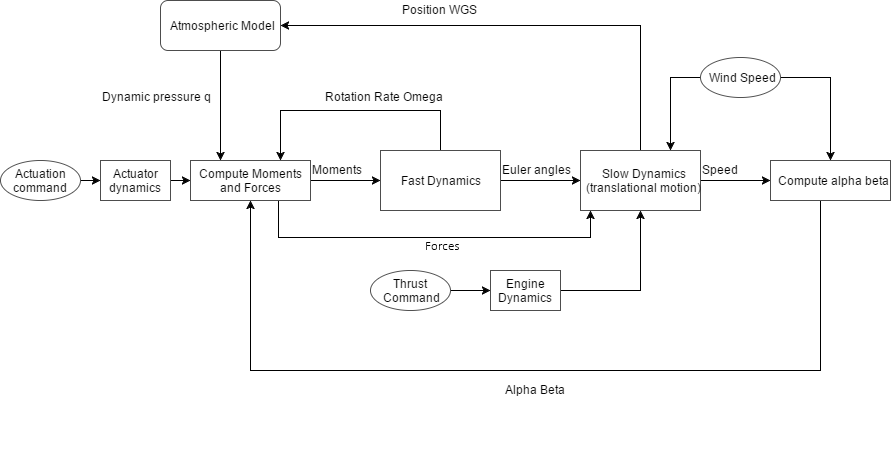
\includegraphics[width=1\textwidth]{Figures/PlaneModel.png}
  \caption[Plane dynamics simulator diagram]{Plane dynamics simulator diagram}
  \label{fig:plane_model}
\end{figure}
 
\subsection{Verification and Validation}
\label{section:model/verification}

To validate such a model in cruise conditions, no actuation was given to the control surfaces, with $\delta_{act_i}=0$.  

Basic test cases to compare the implemented model against other numerical tools (verification) and experimental data (validation)...

\section{Feedback Linearisation}
\label{section:FBL}

\section{Linear Controller}
\label{section:linear_controller}

\subsection{Fast Loop Control}
\label{section:linear_controller/fast_loop}

\subsection{Guidance Control}
\label{section:linear_controller/guidance}

\section{Neural Network}
\label{section:NN}


